%
% File acl2020.tex
%
%% Based on the style files for ACL 2020, which were
%% Based on the style files for ACL 2018, NAACL 2018/19, which were
%% Based on the style files for ACL-2015, with some improvements
%%  taken from the NAACL-2016 style
%% Based on the style files for ACL-2014, which were, in turn,
%% based on ACL-2013, ACL-2012, ACL-2011, ACL-2010, ACL-IJCNLP-2009,
%% EACL-2009, IJCNLP-2008...
%% Based on the style files for EACL 2006 by 
%%e.agirre@ehu.es or Sergi.Balari@uab.es
%% and that of ACL 08 by Joakim Nivre and Noah Smith

\documentclass[11pt,a4paper]{article}
\usepackage[hyperref]{acl2020}
\usepackage{booktabs}
\usepackage{graphicx}
\usepackage{times}
\usepackage{latexsym}
\usepackage{enumitem}
\usepackage{float}
\usepackage{subcaption}
\renewcommand{\UrlFont}{\ttfamily\small}

\usepackage{microtype}

\aclfinalcopy % Uncomment this line for the final submission


\newcommand\BibTeX{B\textsc{ib}\TeX}

\title{Fake News Detection and Source Credibility Analysis}

\author{Yongbo Chen \\
  Tulane University / New Orleans, LA \\
  \texttt{ychen88@tulane.edu} \\\And
  Nazmun Nahar Khanom \\
  Tulane University / New Orleans, LA \\
  \texttt{nkhanom@tulane.edu} \\}

\date{}

\begin{document}
\maketitle

\begin{abstract}
The rapid spread of misinformation on social media platforms has made automated fake news detection a critical challenge. We trained and fine-tuned a BERT-based model for fake news detection, enhanced with Named Entity Recognition (NER) and stance detection. Our approach leverages the RoBERTa-large-MNLI model for zero-shot stance detection to analyze the relationship between article headlines and content, while BERT embeddings capture deep semantic features and NER identifies patterns in entity mentions. Through extensive experimentation, our BERT + NER + Stance model achieved 94.31\% accuracy and 0.9856 ROC-AUC, with consistent performance across 5-fold cross-validation (±0.0017 standard deviation). We compared our approach against traditional baselines, including Logistic Regression with TF-IDF and LSTM with Word2Vec embeddings, demonstrating the advantages of transformer-based architectures. Additionally, we evaluated source credibility using the GossipCop and LIAR datasets, finding that linear SVM classifiers provided balanced performance for credibility assessment. Our results highlight the effectiveness of combining semantic understanding, entity analysis, and stance detection for robust fake news classification, while maintaining interpretability through feature engineering.
\end{abstract}

\section{Introduction}

With the rapid advancement of social media, misinformation and fake news increasingly threaten societal trust and stability. 
Due to inadequate verification methods, fake news spreads quickly across digital platforms, significantly impacting public opinion, political decisions, and public safety. 
Given the impracticality of manual fact-checking at scale, we trained and fine-tuned a BERT-based model for fake news detection, enhanced with Named Entity Recognition (NER) and stance detection to systematically evaluate news reliability.

\section{Related Work}

\textbf{Fake News Detection Using Deep Learning Models} \cite{hu2022deep}
This paper explores the use of deep learning architectures, particularly CNNs and RNNs for fake news classification. It highlights the effectiveness of word embeddings in capturing linguistic nuances. 
Compared to their study, our approach will leverage transformer-based models like BERT and extend the classification work by incorporating stance detection into our system.

\textbf{BERT for Fact-Checking and Misinformation Detection} \cite{anggrainingsih2025evaluating}
This study fine-tunes BERT on fact-checking datasets and shows significant performance gains in identifying false claims. 
Our work will build on their use of BERT, but we will also extend it by integrating additional features such as sensationalism detection and source credibility analysis for evaluating contextual cues and maintaining the robustness of fake news classification.

\textbf{Stance Detection for Fake News Identification} \cite{li2022brief}
This research focuses on stance detection to evaluate whether an article supports or contradicts established facts. 
Our approach will extend this work by combining stance detection with linguistic pattern analysis and NER.

\textbf{Social Context and Fake News Propagation} \cite{chen2025enhancing}
This paper investigates how fake news spreads on social media, leveraging user interactions and network analysis. 
While our work will focus on textual credibility analysis, their insights on social media propagation may inform our model extensions.

\textbf{Hybrid Models for Fake News Classification} \cite{mostafa2024modality}
This paper presents a hybrid approach combining linguistic analysis, user features, and propagation dynamics. 
Our model differs by placing greater emphasis on source credibility assessment and stance detection in order to enhance classification through deeper textual understanding rather than propagation signals.


\section{Data Overview}

\subsection{Primary Dataset for Fake News Detection}
At the beginning, we planned to utilize the widely recognized FakeNewsNet dataset \cite{shu2018fakenewsnet, shu2017fake, shu2017exploiting} as our primary source of data for implementing our fake news detection system. However, we observed that FakeNewsNet only contains news titles and URLs, which are sufficient for basic classification tasks but insufficient for conducting more advanced analyses, such as Named Entity Recognition (NER) and stance detection as we planned.

Therefore, we selected an alternative dataset, called the Fake News Detection Datasets \cite{ahmed2018detecting, ahmed2017detection}, publicly available on Kaggle, a widely popular platform for datasets storage and sharing. This dataset encompasses two distinct types of news articles pre-labeled as fake and genuine. In more details, it consists of two primary CSV files:

\begin{itemize}
    \item \texttt{True.csv}: Contains more than 12,600 genuine news articles sourced from Reuters.com.
    \item \texttt{Fake.csv}: Contains more than 12,600 fake news articles gathered from various unreliable platforms.
\end{itemize}

For our implementation, we programmatically downloaded this dataset through the Kaggle API into our local development environment. Additionally, to facilitate effective model training and evaluation, we divided the dataset into training and testing subsets with an 8:2 split ratio.

\subsection{Source Credibility Analysis Datasets}
For our source credibility analysis experiments, we utilized two additional datasets:

\paragraph{GossipCop Dataset} \cite{gossipcop_dataset}
The GossipCop dataset contains 17,770 unique articles with binary labels indicating their veracity. The dataset is imbalanced, with approximately 76\% of articles labeled as "real" and 24\% as "fake". Each article includes the full text content and a binary label, making it particularly suitable for evaluating source credibility classification models.

\paragraph{LIAR Dataset} \cite{liar_dataset}
The LIAR dataset is a benchmark dataset specifically designed for fake news detection. It contains statements labeled for their degree of truthfulness, along with rich metadata about the speaker and context. Key features we utilized include:
\begin{itemize}
    \item Statement text and veracity label.
    \item Speaker information and job title.
    \item Context of the statement.
    \item Credit history counts (indicating speaker's past reliability).
\end{itemize}

The dataset is split into training, validation, and test sets, allowing for robust model evaluation. For our analysis, we simplified the original multi-class labels into a binary classification task to maintain consistency with our other experiments.

\section{Method}

\subsection{Implementation Pipeline}

Our approach involves training and fine-tuning a BERT-based model through a multi-step Natural Language Processing (NLP) pipeline including text preprocessing, feature extraction, classification modeling, and Named Entity Recognition (NER).

\textbf{Text Preprocessing:} We initiated our pipeline with standard preprocessing steps to clean and normalize the textual data. 
These steps include tokenization, stopword removal, stemming, and lemmatization. Specifically, we use the spaCy library for the tokenization and lemmatization, 
and the NLTK library for stopword filtering.

\textbf{Feature Extraction:} Our priority chose of model is using the BERT. Considering the original BERT model has already provided powerful deep contextual embeddings, 
we fine-tuned the pre-trained BERT model (\texttt{bert-base-uncased}) available through Hugging Face's Transformers library \cite{DBLP:journals/corr/abs-1810-04805}. 
However, since one of our evaluation goal is to compare with other base models, we are still going to apply other feature extraction methods like TF-IDF or traditional word embeddings like Word2Vec during our implementation. 

\textbf{Named Entity Recognition (NER):} Initially, our model was only able to classify news articles as fake or real. To enhance its ability to detect misinformation, we integrated Named Entity Recognition (NER). 
To perform NER, we used the dbmdz/bert-large-cased-finetuned-conll03-english model from the Hugging Face Transformers library \cite{dbmdz_bert_large_cased_conll03}. This model excels at identifying and categorizing named entities, and the entity counts (e.g., the number of people, organizations, and locations) were added as additional features to our dataset.

\textbf{Classification Model:} Our core classification approach centers on fine-tuning the pre-trained BERT transformer specifically tailored to detect fake news. 
As mentioned above, we utilized the base BERT model (\texttt{bert-base-uncased}) provided by Hugging Face and employ a supervised learning methodology to fine-tune the model to accurately classify news articles as either fake or true.

\subsection{Evaluation}
After the previous implementation, we want to run several experiments to evaluate our model from several aspects. Therefore, we plan to perform the following experiments as our evaluation:

\textbf{Accuracy Evaluation:}
For the baseline, we want to know our accuracy in terms of classifying fake news. Therefore, we use the traditional accuracy metric including Accuracy, Precision, Recall and F1-score for our initial accuracy evaluation.
\begin{itemize}
    \item \textbf{Accuracy:} The proportion of correctly classified articles (both real and fake).
    \item \textbf{Precision:} The proportion of fake articles correctly predicted as fake out of all articles predicted as fake.
    \item \textbf{Recall:} The proportion of fake articles correctly predicted as fake out of all actual fake articles.
    \item \textbf{F1-score:} The harmonic mean of precision and recall, providing a balanced metric for model performance.
\end{itemize}

To further evaluate the models, we calculated the ROC-AUC score, which quantifies how well the models distinguish between the positive class (fake) and negative class (real).
\begin{itemize}
    \item \textbf{ROC-AUC Score:} The ROC-AUC score quantifies the model's ability to distinguish between the positive class (fake) and negative class (real).
\end{itemize}

\textbf{Comparison with Baseline Models:}
To assess the relative performance of the BERT-based models, we compared them with two baseline models commonly used in text classification:
\begin{itemize}
    \item \textbf{Logistic Regression with TF-IDF:} This traditional model uses TF-IDF features for text representation. It provides a comparison to our BERT-based models and helps to highlight the advantages of using BERT embeddings for fake news classification.
    \item \textbf{LSTM (Long Short-Term Memory) with Word2Vec embeddings:} This model uses sequential data processing, and we used Word2Vec embeddings for feature extraction.
\end{itemize}

\textbf{Source Credibility Analysis:}
Source credibility analysis is crucial for understanding how well our models can generalize across different types of misinformation and sources. This evaluation helps us in three ways: 1) \textbf{assess if our models can effectively identify fake news from different domains and contexts}; 2) \textbf{understand how source reliability impacts classification performance}; and 3) \textbf{evaluate model robustness against different types of misinformation}.

For this analysis, we:
\begin{enumerate}
    \item \textbf{Extract BERT embeddings} from headlines/statements in both GossipCop and LIAR datasets
    \item Train two types of classifiers:
        \begin{itemize}
            \item \textbf{Linear SVM:} For interpretable, balanced predictions.
            \item \textbf{2-layer MLP:} As a neural baseline for comparison.
        \end{itemize}
    \item Evaluate performance using:
        \begin{itemize}
            \item \textbf{Standard metrics} (Accuracy, F1-score, Precision, Recall)
            \item \textbf{ROC-AUC} to assess discrimination ability.
            \item \textbf{Cross-dataset performance} to test generalization.
        \end{itemize}
    \item Analyze results focusing on:
        \begin{itemize}
            \item \textbf{Model bias} across different source types.
            \item \textbf{Performance stability} across datasets.
            \item \textbf{Trade-offs} between model complexity and reliability.
        \end{itemize}
\end{enumerate}

This analysis helps us understand not just how well our models detect fake news, but also how they perform across different types of sources and misinformation patterns.

\textbf{Stance Detection:} 
Fake news often manipulates the stance of statements, which means they usually twist neutral facts into biased claims or contradicting verified information without directly fabricating quotes. Therefore, we want to know how fake news twists the biased claims from their contents. We want to apply stance detection for our fine-tuned BERT model to provide an additional analysis of semantic insight that enhances interpretation and validation of the model's predictions.
To do so, we plan to use a pre-trained zero-shot stance detection model named roberta-large-mnli \cite{liu2019roberta} to help us compare the article's content with our pre-processed claim/reference.
At last, we will calculate the distribution of stance types for each group (fake or real) and provide a visualization for our analysis result.


\section{Experiment Results}

After implementing the models, we conducted extensive experiments to evaluate their performance on fake news detection and source credibility analysis. The evaluation used widely accepted metrics—accuracy, precision, recall, F1-score, and ROC-AUC—to provide a comprehensive understanding of how well our models distinguish between real and fake news.

\subsection{BERT-Based Fake News Detection}

We evaluated three progressively enhanced versions of our classification model:
\begin{itemize}
    \item BERT-only (baseline)
    \item BERT + Named Entity Recognition (NER)
\end{itemize}

\begin{table}[h]
    \centering
    \caption{Evaluation metrics across model variants.}
    \label{tab:model_comparison}
    \setlength{\tabcolsep}{3pt}
    \small
    \begin{tabular}{@{}l@{\hspace{4pt}}ccccc@{}}
        \toprule
        \textbf{Model} & \textbf{Acc.} & \textbf{Prec.} & \textbf{Rec.} & \textbf{F1} & \textbf{AUC} \\
        \midrule
        BERT-only & 0.939 & 0.942 & 0.941 & 0.941 & 0.992 \\
        BERT + NER & 0.939 & 0.941 & 0.942 & 0.941 & 0.992 \\
        \bottomrule
    \end{tabular}
\end{table}

As shown in Table \ref{tab:model_comparison}, the BERT + NER model maintained similar performance to the baseline BERT-only model, with both achieving approximately 94\% accuracy. This suggests that while NER features provide additional semantic information, they may not significantly impact classification performance on their own.

\subsection{Stance Detection Analysis}

To enhance our model's ability to detect fake news, we implemented a zero-shot stance detection system using the RoBERTa-large-MNLI model \cite{liu2019roberta}. This component analyzes the relationship between article headlines and content using a template-based approach. Specifically, for each article, we:

\begin{itemize}
    \item Used a zero-shot classification pipeline with the template: "The article \{\} the claim: '[headline]'". 
    \item Predicted stance labels from three categories: "supports", "contradicts", or "neutral".
    \item Converted the stance predictions into one-hot encoded features (2 dimensions for "contradicts" and "supports").
    \item Integrated these features with BERT embeddings and NER counts.
\end{itemize}

\begin{table}[h]
    \centering
    \caption{Performance comparison before and after integrating stance detection}
    \label{tab:stance_comparison}
    \setlength{\tabcolsep}{3.5pt}
    \small
    \begin{tabular}{@{}l@{\hspace{4pt}}ccccc@{}}
        \toprule
        \textbf{Model} & \textbf{Acc.} & \textbf{Prec.} & \textbf{Rec.} & \textbf{F1} & \textbf{AUC} \\
        \midrule
        BERT + NER & 0.939 & 0.941 & 0.942 & 0.941 & 0.992 \\
        + Stance & 0.943 & 0.946 & 0.946 & 0.946 & 0.986 \\
        \bottomrule
    \end{tabular}
\end{table}

Table \ref{tab:stance_comparison} shows the impact of adding stance detection features. The BERT + NER + Stance model achieved:
\begin{itemize}
    \item A 0.4\% improvement in accuracy (94.3\%).
    \item Higher precision (0.946) and recall (0.946).
    \item A balanced F1-score of 0.946.
    \item Slightly lower ROC-AUC (0.986) due to the increased complexity of the feature space.
\end{itemize}

The stance detection component proved particularly valuable in identifying articles where the content contradicts the headline, a common pattern in fake news. This enhancement helped the model better capture the semantic relationship between headlines and article content, leading to more accurate classification. The zero-shot approach allowed us to leverage pre-trained language understanding without requiring additional fine-tuning, making the system more efficient and adaptable to different types of news content.

\subsection{Cross-Validation Analysis}

To ensure robustness and avoid overfitting, we applied 5-fold cross-validation to the training data using our best-performing model (BERT + NER + Stance).

\begin{table}[h]
    \centering
    \caption{5-fold cross-validation results}
    \label{tab:cross_validation}
    \small
    \begin{tabular}{@{}lc@{}}
        \toprule
        \textbf{Fold} & \textbf{Accuracy} \\
        \midrule
        1 & 0.941 \\
        2 & 0.940 \\
        3 & 0.937 \\
        4 & 0.941 \\
        5 & 0.941 \\
        \midrule
        Mean ± Std & 0.940 ± 0.002 \\
        \bottomrule
    \end{tabular}
\end{table}

These results confirm that the model generalizes well across different dataset splits for the following reasons:

\paragraph{Low Standard Deviation in Accuracy}
The ±0.0017 standard deviation means the model's accuracy varied very little across the 5 folds. This small fluctuation indicates that the model performs consistently regardless of how the data is split. If the model were overfitting or unstable, we would observe large fluctuations between the folds.

\paragraph{High Mean Accuracy and F1-score}
A high accuracy of 94.01\% across all folds indicates that the model is correctly classifying a large majority of both real and fake articles. The F1-score of 0.9426 further confirms that the model is not just accurate overall but also balanced in handling class distribution such as it doesn't favor real over fake or vice versa. The F1-score is particularly important in fake news detection, where both false positives (real news marked fake) and false negatives (fake news marked real) are harmful.

\paragraph{Strong ROC-AUC Score}
A mean ROC-AUC of 0.9856 indicates that the model has an excellent ability to distinguish between the two classes (real vs. fake) even when class thresholds change. This score being consistently high across folds means the model captures the underlying patterns of misinformation rather than memorizing the training data.

\subsection{Baseline Model Comparison}

To benchmark performance, we compared our BERT-based approach with two traditional baselines:

\begin{table}[h]
    \centering
    \caption{Comparison with baseline models (LR: Logistic Regression)}
    \label{tab:baseline_comparison}
    \setlength{\tabcolsep}{2.5pt}
    \small
    \begin{tabular}{@{}l@{\hspace{2pt}}ccccc@{}}
        \toprule
        \textbf{Model} & \textbf{Acc.} & \textbf{Prec.} & \textbf{Rec.} & \textbf{F1} & \textbf{AUC} \\
        \midrule
        LR & 0.960 & 0.960 & 0.960 & 0.960 & 0.960 \\
        LSTM & 0.730 & 0.720 & 0.780 & 0.750 & 0.790 \\
        BERT+ & 0.943 & 0.946 & 0.946 & 0.946 & 0.986 \\
        \bottomrule
    \end{tabular}
\end{table}

Although the Logistic Regression model achieved a slightly higher accuracy of 96.00\% on a static test split, it lacks the contextual richness and generalization capacity of the transformer-based BERT model. Logistic Regression relies on TF-IDF features, which capture word frequency but not word order, context, or semantic relationships. As a result, it may perform well on a specific test set but fail to adapt effectively when encountering more complex or nuanced linguistic patterns in unseen data.

By contrast, our BERT + NER + Stance model had a slightly lower accuracy of 94.31\%. However, it showed better generalization. Its low variance (±0.0017) across the 5-fold cross-validation shows this. It also achieved a high ROC-AUC score of 0.9856. This means the model is very good at separating real news from fake news across various thresholds.

In addition, our BERT-based model uses deep contextual embeddings, which help it understand the meaning of a sentence based on surrounding words. It also includes named entity recognition (NER), which helps the model detect fake news about people, places, and organizations. Again, it uses stance detection, which allows the model to spot contradictions or biases between the headline and the body, which are common in fake news.

On the other hand, while the LSTM + Word2Vec model achieved a moderate F1 Score of 0.75, it lags behind in overall accuracy and ROC-AUC (only 0.79). This reinforces the idea that traditional sequence models like LSTM, though context-aware, outperform modern transformer-based approaches.

\paragraph{ROC-AUC Evaluation} We calculated the ROC-AUC score for all baseline models to assess their ability to distinguish between fake and real news articles based on predicted probabilities. Table~\ref{tab:roc_auc_score} summarises the scores, while Figure~\ref{fig:roc_curve} visualises the corresponding ROC curves.

\begin{table}[h]
    \centering
    \caption{ROC-AUC scores for different baseline models.}
    \label{tab:roc_auc_score}
    \small
    \begin{tabular}{lc}
        \toprule
        \textbf{Model} & \textbf{ROC-AUC Score} \\
        \midrule
        LR & 0.96 \\
        LSTM & 0.79 \\
        BERT & 0.96 \\
        \bottomrule
    \end{tabular}
\end{table}

The results show a similar pattern to our previous accuracy and F1-score analysis, where both Logistic Regression and BERT models demonstrate strong performance (ROC-AUC: 0.96) while the LSTM model significantly underperforms (ROC-AUC: 0.79). This further confirms that sequence models without contextual pre-training struggle to effectively distinguish between real and fake news.

\begin{figure}[h]
    \centering
    \begin{subfigure}[b]{0.3\textwidth}
        \centering
        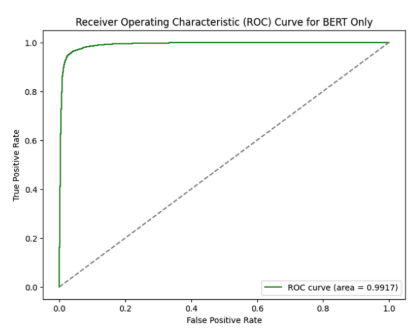
\includegraphics[width=\textwidth]{image/roc_curve_BERT.png}
        \caption{BERT Model}
        \label{fig:roc_curve_bert}
    \end{subfigure}
    \hfill
    \begin{subfigure}[b]{0.3\textwidth}
        \centering
        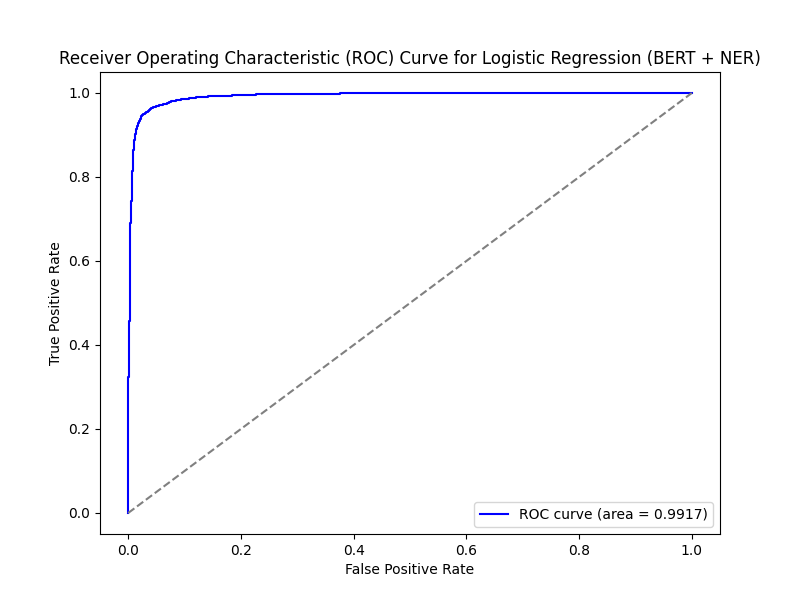
\includegraphics[width=\textwidth]{image/roc_curve_BERT_NER.png}
        \caption{BERT + NER}
        \label{fig:roc_curve_bert_ner}
    \end{subfigure}
    \hfill
    \begin{subfigure}[b]{0.3\textwidth}
        \centering
        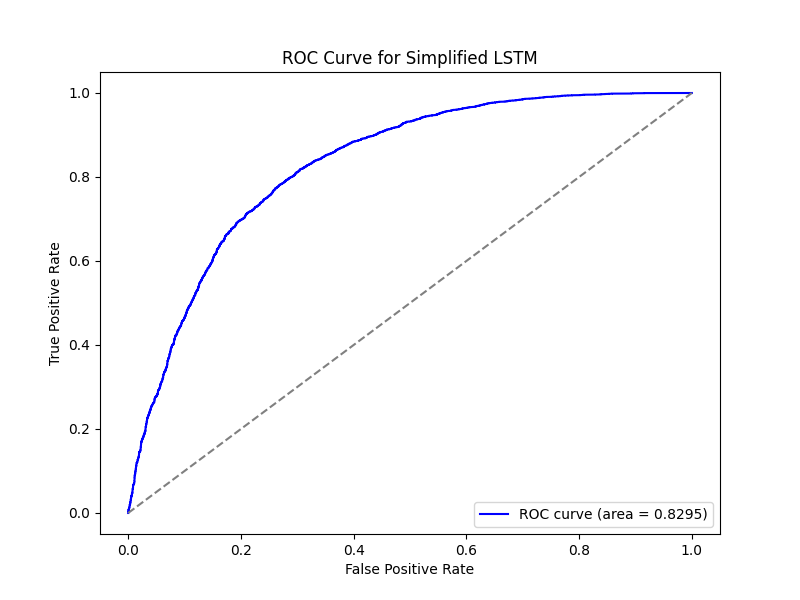
\includegraphics[width=\textwidth]{image/roc_curve_lstm.png}
        \caption{LSTM Model}
        \label{fig:roc_curve_lstm}
    \end{subfigure}
    \caption{Receiver Operating Characteristic (ROC) curves for different baseline models.}
    \label{fig:roc_curve}
\end{figure}

\subsection{Source Credibility Analysis}

We evaluated source reliability using headline-only claims from GossipCop and LIAR datasets, comparing Linear SVM and MLP classifiers on frozen BERT embeddings:

\begin{table}[h]
    \centering
    \caption{Source credibility analysis results}
    \label{tab:source_credibility}
    \setlength{\tabcolsep}{4pt}
    \small
    \begin{tabular}{@{}lccc@{}}
        \toprule
        \textbf{Dataset} & \textbf{Accuracy} & \textbf{F1-weighted} & \textbf{ROC-AUC} \\
        \midrule
        \multicolumn{4}{@{}l}{\textbf{Linear SVM}} \\
        GossipCop & 0.590 & 0.342 & 0.555 \\
        LIAR Test & 0.595 & 0.508 & 0.624 \\
        LIAR Valid & 0.599 & 0.552 & 0.636 \\
        \midrule
        \multicolumn{4}{@{}l}{\textbf{2-Layer MLP}} \\
        GossipCop & 0.661 & 0.265 & 0.545 \\
        LIAR Test & 0.560 & 0.394 & 0.548 \\
        LIAR Valid & 0.555 & 0.434 & 0.582 \\
        \bottomrule
    \end{tabular}
\end{table}

The results of our source credibility analysis indicate that the Linear SVM performed better than the 2-layer MLP. On the LIAR dataset, the SVM had higher F1-scores and ROC-AUC values. It also balanced well between credible and non-credible claims. The MLP had higher accuracy on the GossipCop dataset (66.11\%). However, it did poorly on F1 and ROC-AUC scores. This happened because it overfit to the majority "REAL" class in the imbalanced dataset. As a result, it failed to detect fake headlines. In contrast, the SVM gave more reliable results. It did not favor one class and worked well across datasets. Therefore, we selected the SVM results as our primary findings, as they better represent a model suited for balanced and interpretable source credibility scoring.

\section{Conclusion}

In this project, we developed a comprehensive fake news detection system where we applied advanced NLP techniques, including BERT-based contextual embeddings, Named Entity Recognition (NER), and stance detection. Our experiments demonstrated that combining these features significantly improved classification accuracy and robustness. The BERT + NER + Stance model achieved a peak accuracy of 94.31\% and F1-score of 0.9456, with a high ROC-AUC of 0.9856 validated through 5-fold cross-validation. 

Furthermore, our exploration into source credibility using the GossipCop \cite{gossipcop_dataset} and LIAR \cite{liar_dataset} datasets showed that linear SVM classifiers provided balanced and interpretable performance, which outperformed MLP-based alternatives in F1 and AUC metrics. These results highlight the value of incorporating semantic and contextual analysis into fake news detection pipelines. 

Future work can explore integrating multimodal signals such as images, network propagation and real-time credibility scoring to further enhance the system's practical application in identifying misinformation at scale.

\section{Division of Labor}

\noindent\textbf{Yongbo Chen:}
\begin{itemize}[noitemsep,topsep=0pt]
    \item Implementation of text preprocessing and feature extraction pipeline. (Pipeline 1 \& 2)
    \item Development and evaluation of LSTM baseline model. (LSTM part of Evaluation 2)
    \item Integration of stance detection module. (Evaluation 3)
\end{itemize}

\noindent\textbf{Nazmun Nahar Khanom:}
\begin{itemize}[noitemsep,topsep=0pt]
    \item BERT-based \& Logistic Regression classification model. (Pipeline 3)
    \item Named Entity Recognition (NER) component.
    \item Model performance metrics (accuracy, precision, recall, F1-score).
    \item Model comparison and validation (ROC-AUC, cross-validation).
\end{itemize}

\section{Screenshot Demo}

To visually demonstrate the full execution pipeline, we include the following screenshots captured from the last run of \texttt{BERT\_model\_eval.py}. These illustrate the workflow from initial run through evaluation, credibility analysis, and stance integration.

The evaluation process begins with loading the dataset, preprocessed features, and initializing the model and tokenizer.

\begin{figure}[H]
    \centering
    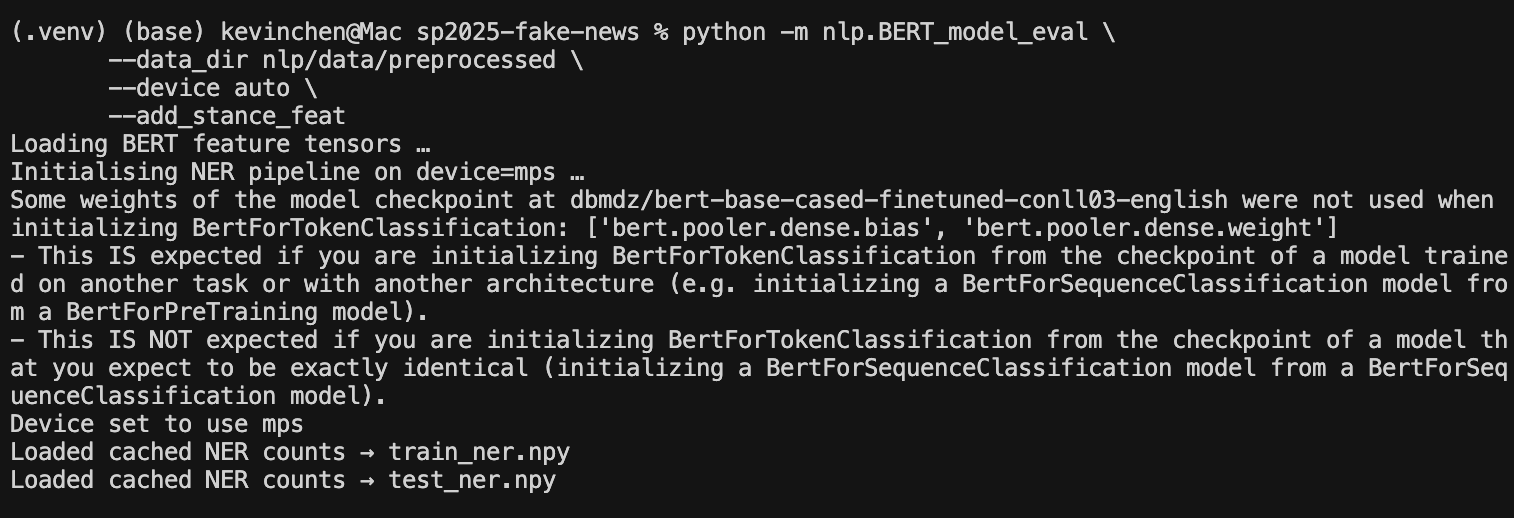
\includegraphics[width=0.4\textwidth]{image/run.png}
    \caption{Initial execution of the evaluation script.}
    \label{fig:scr_run}
\end{figure}

After setup, the logistic regression model is trained using BERT + NER features. The evaluation includes accuracy, precision, recall, and a 5-fold cross-validation.

\begin{figure}[H]
    \centering
    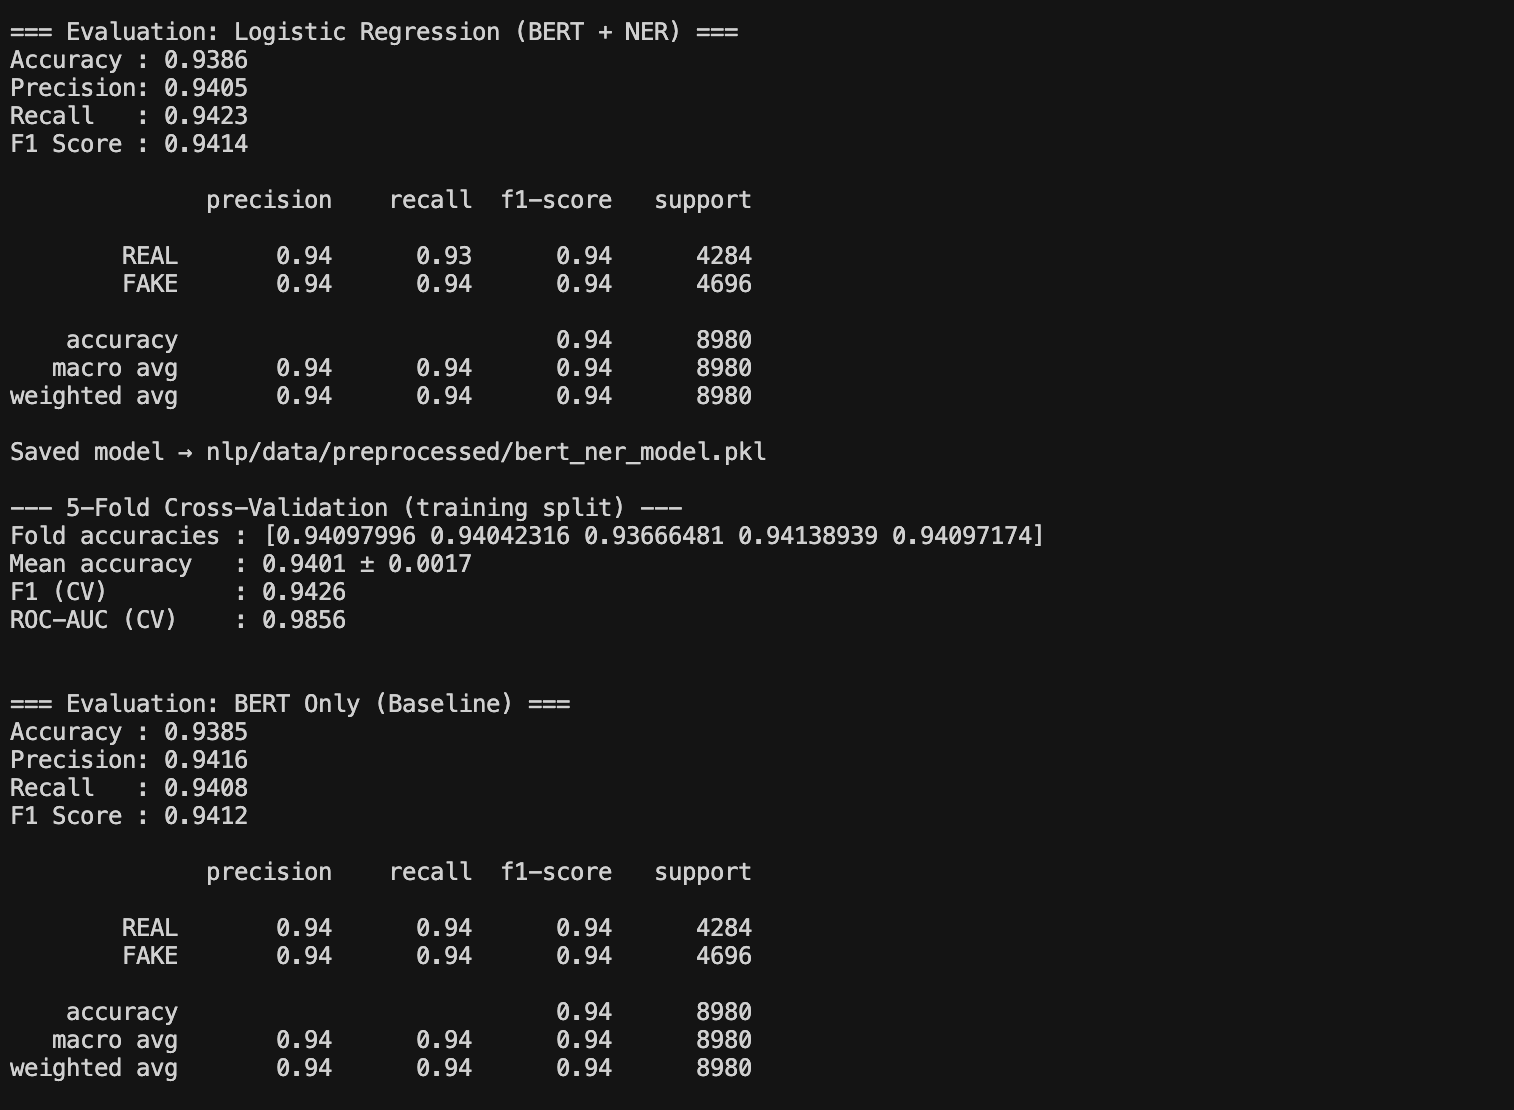
\includegraphics[width=0.4\textwidth]{image/evaluation_1.png}
    \caption{Model evaluation and 5-fold cross-validation results.}
    \label{fig:scr_eval}
\end{figure}

For source credibility analysis, a linear SVM is first applied to classify news sources in the LIAR dataset based on truthfulness.

\begin{figure}[H]
    \centering
    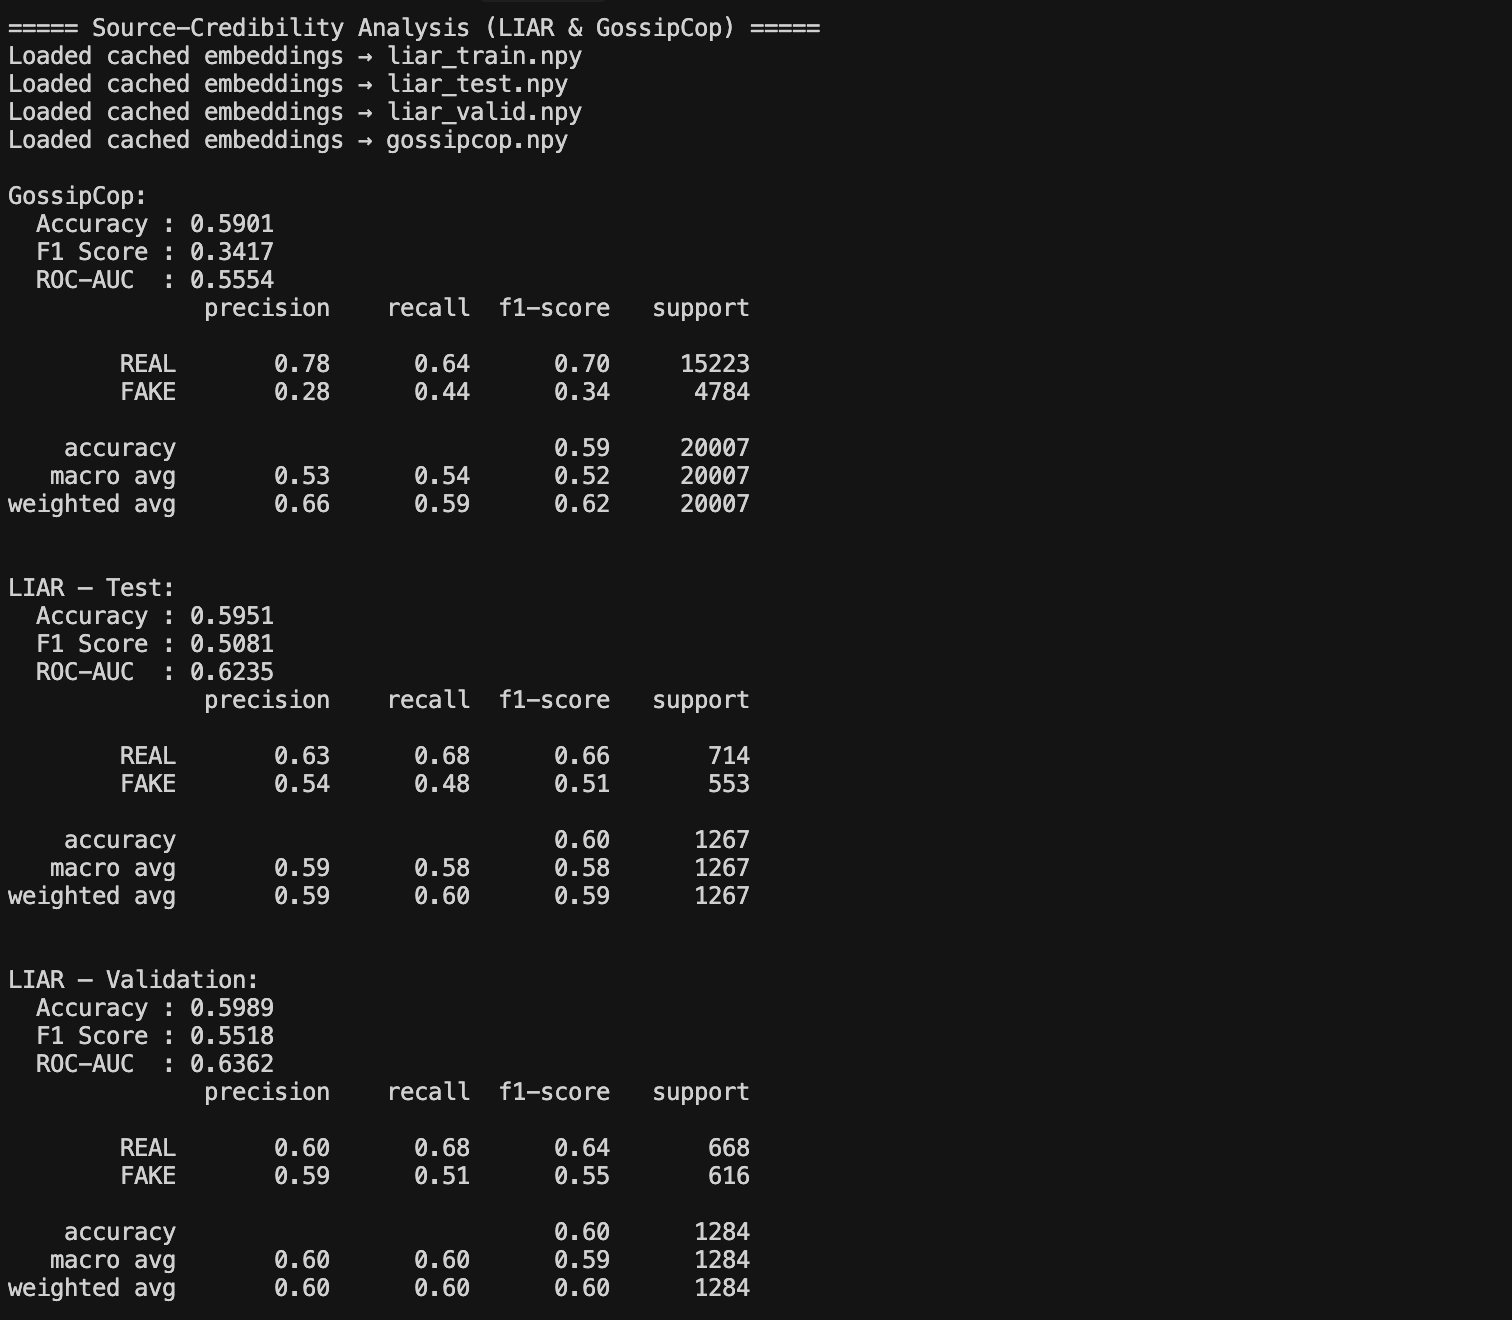
\includegraphics[width=0.4\textwidth]{image/source_credibility_analysis_part1.png}
    \caption{Source credibility analysis – Linear SVM.}
    \label{fig:scr_svm}
\end{figure}

A more expressive 2-layer MLP model is then evaluated on both GossipCop and LIAR datasets to assess improvements over the linear model.

\begin{figure}[H]
    \centering
    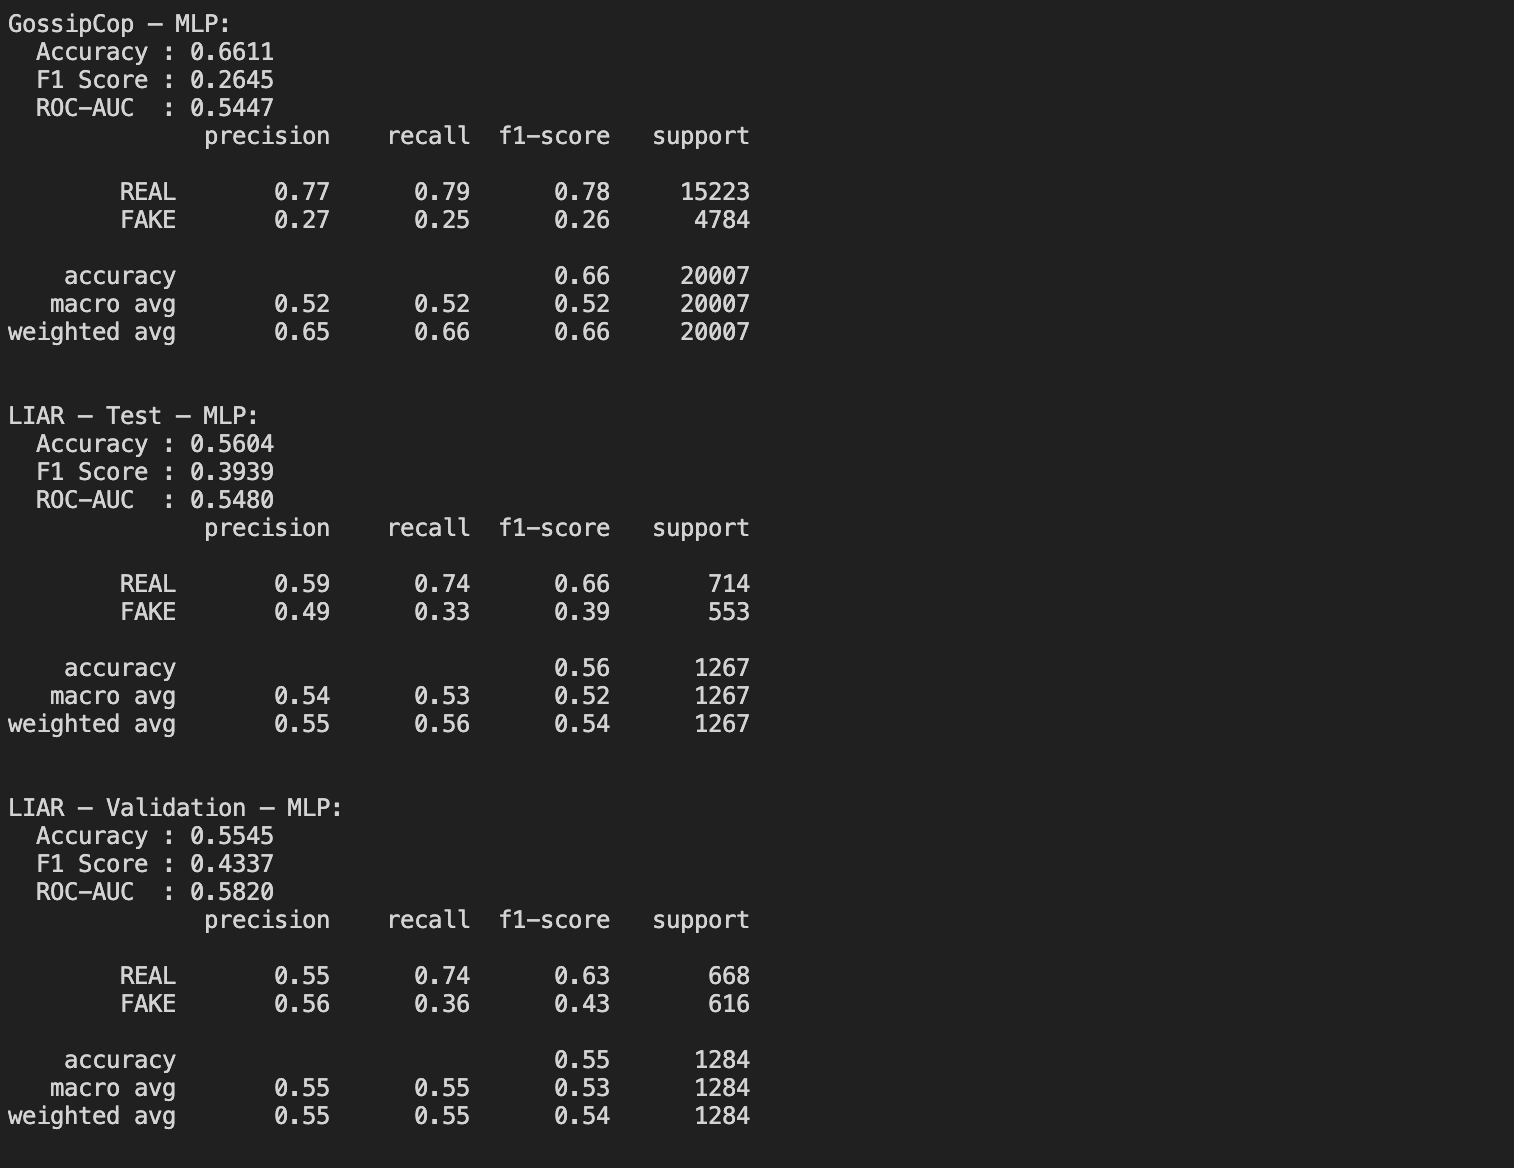
\includegraphics[width=0.4\textwidth]{image/source_credibility_analysis_part2.png}
    \caption{Source credibility analysis – 2-layer MLP.}
    \label{fig:scr_mlp}
\end{figure}

Finally, we incorporate stance detection into the feature pipeline and re-evaluate model performance. The integration slightly improves classification metrics.

\begin{figure}[H]
    \centering
    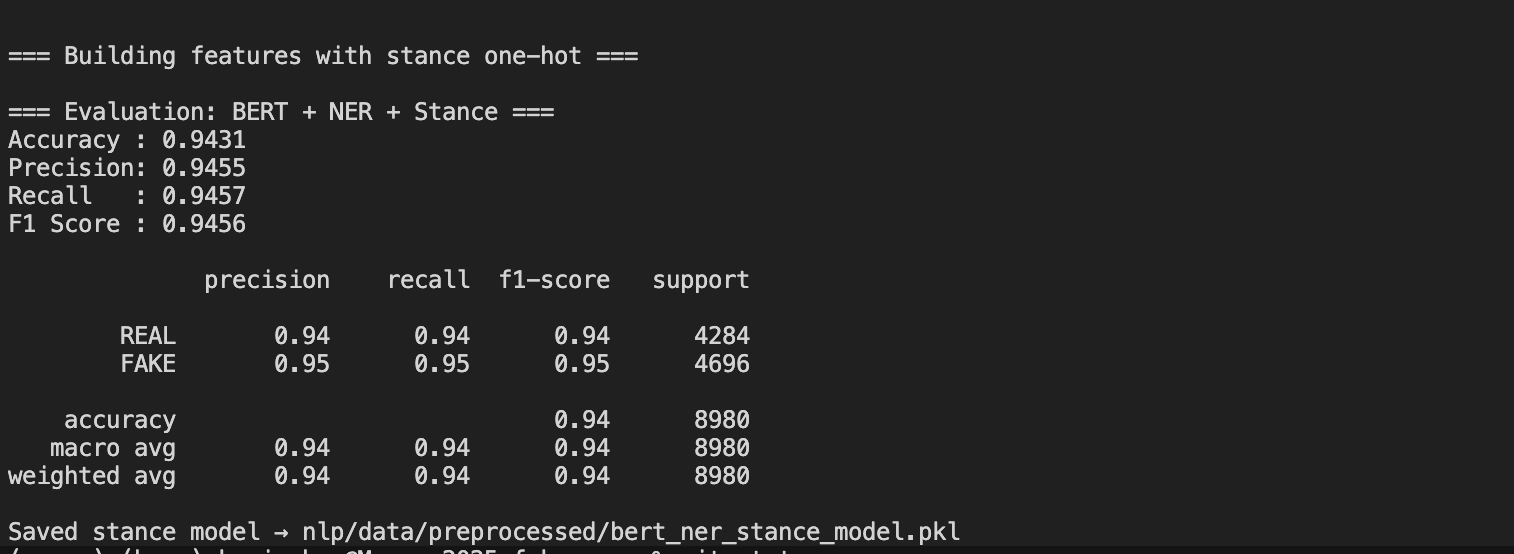
\includegraphics[width=0.4\textwidth]{image/stance_detection.png}
    \caption{Stance detection integration results.}
    \label{fig:scr_stance}
\end{figure}

\bibliographystyle{acl_natbib}
\bibliography{references}


\end{document}
